
%
%
%  $Description: Author guidelines and sample document in LaTeX 2.09$ 
%
%  $Author: ienne $
%  $Date: 1995/09/15 15:20:59 $
%  $Revision: 1.4 $
%

\documentclass[times, 10pt,twocolumn]{article} 
\usepackage{latex8}
\usepackage{times}
\usepackage{pdfpages}
\usepackage{float}
\usepackage{graphicx}
\usepackage{enumitem}
\usepackage{comment}
\usepackage{caption}
\usepackage{subcaption}
\usepackage[scaled=1]{helvet}
\DeclareCaptionFont{xipt}{\fontsize{10}{11}\sf\selectfont}
\DeclareCaptionLabelSeparator{bar}{.\space}
\captionsetup{labelsep=bar}
 \captionsetup[figure]{font=xipt,labelfont=bf}
%\documentstyle[times,art10,twocolumn,latex8]{article}

%------------------------------------------------------------------------- 
% take the % away on next line to produce the final camera-ready version 
\pagestyle{empty}

%-------------------------------------------------------------------------
%Macros para  imagenes (png, jpg)
\newcommand{\img}[4]{
   \begin{figure}[H]
   	   \centering
   	%Imagen principal del documento
       \includegraphics[scale=#1]{Img/#2}
       \caption{#3}
   	   \label{#4}
       \end{figure}
   }


 \newcommand{\Img}[5]{
   \begin{figure}[H]
   	   \centering
   	%Imagen principal del documento
       \includegraphics[width=#1, height=#2]{Img/#3}
       \caption{ \centering \textbf{\small #4}}
       \label{#5}
   
       \end{figure}
   } 
 \newcommand{\Imgr}[6]{
   \begin{figure}[H]
   	   \centering
   	%Imagen principal del documento
       \includegraphics[angle=#1, origin=tr, width=#2, height=#3]{Img/#4}
       \caption{ \centering \textbf{\small #5}}
       \label{#6}
   
       \end{figure}
   } 
%------------------------------------------------------------------------
%Contadores
\newcounter{module}
\setcounter{module}{1}

%-------------------------------------------------------------------------
\begin{document}

\title{Diseño y Desarrollo de una Placa Entrenadora del Microcontrolador PIC18F45K50}
\author{Francisco Javier Mendoza Bautista\\
Universidad de Guanajuato\\ Departamento de Comunicaciones y Electrónica \\  
Salamanca/Guanajuato, México\\fj.mendozabautista@ugto.mx\\
% For a paper whose authors are all at the same institution, 
% omit the following lines up until the closing ``}''.
% Additional authors and addresses can be added with ``\and'', 
% just like the second author.
\and
Second Author\\
Institution2\\
First line of institution2 address\\ Second line of institution2 address\\ 
SecondAuthor@institution2.com\\
}

\maketitle
\thispagestyle{empty}

\begin{abstract} 
El campo de la Ingeniería en Comunicaciones y Electrónica es pilar para los avances tecnológicos cuyo crecimiento y desarrollo ha sido exponencial en los últimos años; en este contexto, los microcontroladores juegan un papel importante ya que son versátiles y pueden ser programados para que ejecuten tareas según sea su uso. Resulta esencial desarrollar habilidades en el software del microcontrolador y utilizar un hardware que nos permita comprobar el software escrito. En este estudio se presenta la evolución de una placa de prueba y desarrollo en la que se puede programar un microcontrolador PIC18F4550 o un PIC18F45K50, lo que permite mayor flexibilidad para trabajar con módulos dentro de la placa. El conjunto propuesto incluye pantalla tipo OLED, conjunto de leds, teclado matricial, 7 segmentos unificados, bluetooth, conexión WiFi, grupo de botones, puerto USB tipo C, buzzer, potenciómetro para el ADC, sistema de alimentación externa, módulo de radiofrecuencia y la posibilidad de programar por medio de PIKIT3 o vía USB.\\

\textbf{Palabras clave:} ingeniería electrónica, microcontroladores, PIC18F45K50, placa de desarrollo, diseño PCB
\end{abstract}
\vspace*{-0.6cm}
%------------------------------------------------------------------------- 
\Section{Introducción}
\vspace*{-0.1cm}
A  medida que la tecnología avanza, profesionistas y estudiantes de Ingeniería Electrónica estamos comprometidos a seguir su ritmo; debido a esto, es necesario incorporar herramientas que nos permitan crecer y desarrollar estas nuevas tecnologías. En este contexto surgen los microcontroladores para facilitar nuestra vida cotidiana.

Un microcontrolador es un circuito integrado programable que se ha colocado en varios sectores del mercado para realizar numerosas aplicaciones, permitiendo el crecimiento acelerado de la tecnología de control.

Si bien, no podemos mencionar con precisión acerca del origen de estos, se conoce que la empresa Microchip Technology Inc. es líder en la fabricación de los Controles de Interfaz Periférica (PIC); su éxito radica en que tienen una gran variedad de productos a bajo costo, son versátiles
y poseen una amplia disponibilidad de herramientas para su correcta programación.~\cite{ex1}
%1. RELACIONAR CON LA PLACA DE DESARROLLO
%2. PLANTEAMIENTO DEL PROBLEMA. (Señala un vacío en la información respecto al objeto)
%3. OBJETIVO DE ESTE ESTUDIO. ¿PARA QUÉ SE CONSTRUYE? PROPUESTA. Aquí puedes mencionar acerca del desarrollo de tus tres versiones. ¿Por qué tres versiones? ¿Qué se espera de la placa versión 3?
% La tecnología crece, industria y demás debe mantenerse al tanto. Existen equipos que se actualizan di a día.

Los microcontroladores generalmente se suman a las placas de desarrollo donde por medio de lenguaje de programación se pueden escribir las instrucciones para que estos las ejecuten; por lo tanto, es necesario utilizar un hardware que nos permita comprobar el software escrito.

En un principio, la idea de construir una placa de desarrollo fue para apoyar a los estudiantes que estuvieran cursando materias en programación de microcontroladores o diseño de Placa de Circuito Impreso (PCB), pues existe poca información respecto al tema; es posible que esto se deba a la falta de empatía a las necesidades que presenta un estudiante.

Con respecto al software de automatización del diseño electrónico (EDA) para diseño PCB, existe una gran variedad, pero desafortunadamente, la mayoría son de tipo privativo, lo cual limita tanto su acceso como el futuro de la placa de desarrollo en las aplicaciones que se propongan; por esta razón se optó por usar un software libre llamado KICAD el cual cuenta con un entorno bastante completo y es de gran respaldo en la comunidad.~\cite{ex2}

Este proyecto inicia con la Versión 1.0, un diseño de dimensiones grandes que resulta poco accesible para diferentes aplicaciones, pero cumple satisfactoriamente con su objetivo principal; este contaba con lo necesario para poder cumplir al margen con proyectos escolares.

Posteriormente, se pensó mejorar este proyecto, no solo enfocado a la escuela si no también a la industria con el fin de brindarle una herramienta más a los
egresados de la carrera de Ingeniería Electrónica quienes constantemente se enfrentan a problemas técnicos para la inserción al campo laboral; para esto,
se añadieron nuevos sensores que se adaptan a las aplicaciones de la industria y se logró reducir las dimensiones de la placa para dar paso a la Versión 2.0

Por último, se trabajó la Versión 3.0 donde se podrán desarrollar aplicaciones para diversas áreas del conocimiento como son la electrónica, óptica inteligencia artificial, biomédica, entre otras. En otras palabras, esta placa pasa de tener una única función a ser multifuncional.

%-------------------------------------------------------------------------
\Section{Materiales y métodos}

\SubSection{PIC18F45K50}

PIC18F45K50 es un circuito integrado programable, también llamado microcontrolador, perteneciente a la familia de PIC18 y que puede ejecutar tareas programadas según sea su aplicación en los distintos sectores: industria, automoción, electrónica de consumo, entre otros.

Entre las características a destacar del PIC18F45K50 se encuentran su capacidad para soportar voltajes de operación de 4.2V hasta 5.5V, módulos de comunicación serial UART, A/E/USART, SPI, $I^{2}$C, módulo MSSP (SPI-I2C), 13 canales de ADC trabajando a 10 bits, 35 pines I/O disponibles, 2 comparadores análogos, una memoria tipo EEPROM de 256 bytes, memoria flash de 32 kB y frecuencia máxima de 48MHz~\cite{ex3}; suficientes para posicionar a este microcontrolador como uno de los más completos y preferidos del momento, además de que su precio es considerablemente menor comparado con otros disponibles en el mercado.

%-------------------------------------------------------------------------

%-------------------------------------------------------------------------
%Primera versión

\SubSection{Placa entrenadora Versión 1.0}
Consistió en el diseño de un circuito de prueba al que denominamos versión 1.0; de inicio se dispuso de un software de uso libre para la automatización del diseño electrónico de los diagramas de circuito, los cuales incluyeron los siguientes componentes: un módulo robusto de alimentación, botón RESET, led indicador de alimentación ya sea vía PIKIT3 o USB, salida por PIN del PIC18F45K50 y módulo de sensores (conformado por HC-06, NRF24L01, 4 leds, teclado, buzzer, y un potenciómetro para regular el brillo de la pantalla LCD). 

La primera versión contó con tecnología through hole (THT), favoreciendo las pruebas de fuentes de alimentación a las que se sometieron cada uno de los módulos por separado. Posteriormente, para evaluar su correcto funcionamiento integral, se utilizó un
código DEMO para la realización simultánea de pruebas de comunicación vía serial, SPI y $I^{2}$C, como se muestra en la Fig.~\ref{fig:1}

\Img{7.5cm}{7.0cm}{Primera_Version.pdf}{Diagrama de circuito Verión 1.0}{fig:1}

Después de verificar el procedimiento anterior, se siguió con el dibujo del circuito impreso teniendo como premisa de diseño no exceder un tamaño de 10x10cm a fin de presentar un producto compacto y atractivo, de fácil acceso y uso para el usuario. En la Fig.~\ref{fig:2} se muestra el diagrama de circuito impreso propuesto.

\Img{8.5cm}{8.5cm}{primera_version_pcb}{Diagrama de circuito impreso Versión 1.0}{fig:2}
%\newpage
Como método para evitar errores de diseño al dibujar el circuito impreso, nos apoyamos en la visualización 3D que se puede apreciar en la Fig.~\ref{fig:3} y en el estudio minucioso del modelo.

\Img{8.5cm}{7.5cm}{primera_version_3d}{Modelo 3D de circuito impreso Versión 1.0}{fig:3} 

Una vez obtenida la alineación de todos los componentes, se imprimió el diseño del circuito en la placa que resulta en la forma final que se advierte en la Fig.~\ref{fig:4}

Gracias a este diseño se comprobó que cada uno de los módulos funcionaba correctamente.
\Img{8.5cm}{7.5cm}{primera_version_final}{Placa de desarrollo Versión 1.0}{fig:4} 


%-------------------------------------------------------------------------

%Segunda versión
\SubSection{Placa entranadora Versión 2.0}
\vspace{-0.2cm}
Esta nueva versión parte del diseño descrito anteriormente, removiéndose los elementos THT para sustituirlos por tecnología de montaje superficial (SMD); asimismo, se añadieron: 2 salidas por PIN del PIC18F45K50, salidas de 3.3V y 5V, 7leds que cubren el PORTA, un control de leds, un control buzzer, led indicador de activación del buzzer, potenciómetro para ADC, control de ADC y brillo automático en la pantalla LCD. Esta serie de cambios permitió la Versión 2.0 representada inicialmente en el diagrama de la Fig.~\ref{fig:5}

\Img{8.5cm}{7.0cm}{Segunda_Version}{Diagrama de circuito Versión 2.0}{fig:5}
Por consecuencia se ajustó el dibujo del circuito impreso para agregar los nuevos elementos, sin embargo, cabe destacar que las medidas de diseño se redujeron a 9.017cm x 9.906cm como se muestra en la Fig.~\ref{fig:6}

\Img{8.5cm}{8.5cm}{segunda_version_pcb}{Diagrama de circuito impreso Versión 2.0}{fig:6}


Nuevamente recurrimos al análisis a partir de un modelo 3D para evitar posibles fallas en el dibujo del circuito impreso, como se puede apreciar en la Fig.~\ref{fig:7}

\begin{figure}[H]
  \begin{subfigure}[b]{0.4\columnwidth}
    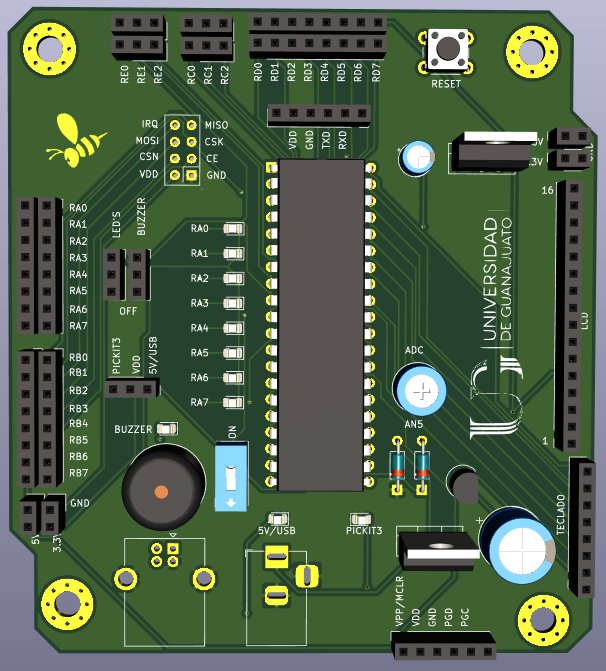
\includegraphics[width=4.3cm, height=5.0cm]{Img/segunda_version_3d.png}
    % \caption{Primera imagen.}
    %\label{fig:f13}
  \end{subfigure}
  \hspace{0.7cm}
  \begin{subfigure}[b]{0.4\columnwidth}
    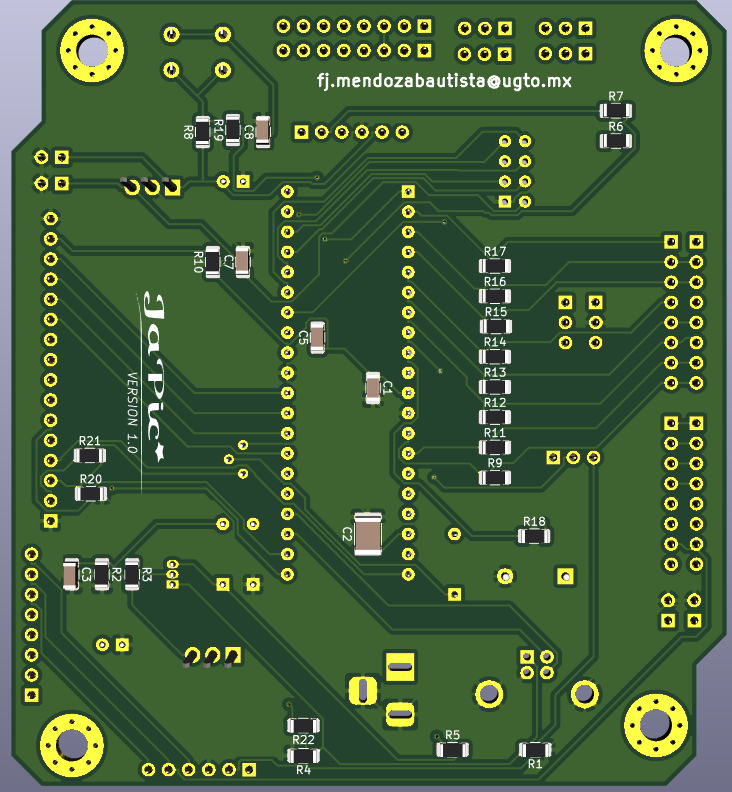
\includegraphics[width=4.3cm, height=5.0cm]{Img/segunda_version_pcb_b.png}
   % \caption{Segunda imagen.}
    %\label{fig:f23}
  \end{subfigure}
   \caption{\centering \textbf{Modelo 3D de circuito impreso Versión 2.0}} 
   \label{fig:7}
 \end{figure}
%\Img{7.2cm}{6.2cm}{segunda_version_3d}{Modelo 3D de circuito impreso Versión 2.0 capa superior}{fig:7}
%\Img{7.2cm}{6.2cm}{segunda_version_pcb_b}{Modelo 3D de circuito impreso Versión 2.0 capa inferior}{fig:6}


Una vez obtenida la alineación de todos los componentes, se imprimió el diseño del circuito en la placa que resulta en la forma final que se advierte en la Fig.~\ref{fig:8}
\Img{8.5cm}{8.5cm}{segunda_version_final}{Placa de desarrollo Versión 2.0}{fig:8}


%------------------------------------------------------------------------- 
%Tercera versión
\SubSection{Placa entrenadora Versión 3.0}
\vspace{-0.1cm}
En la tercera y más reciente versión se agregaron un puerto USB tipo C, un nuevo sistema de alimentación, pantalla OLED, 3 push button para interrupciones, modo de programación con bootloader y 3 display de 7 segmentos unificados; todo esto se dispone en el diagrama de la Fig.~\ref{fig:9}
\Img{8.5cm}{7.0cm}{Tercera_Version}{Diagrama de circuito Versión 3.0}{fig:9}

Continuando con el diseño del circuito impreso, una vez más se consiguió reducir las medidas de
construcción de la placa, quedando de 7.080 x 8.050 cm. Los componentes de la placa de entrenamiento propuesta en este estudio se describen a continuación.

\Img{7.5cm}{7.0cm}{tercera_version_pcb}{Diagrama de circuito impreso Versión 3.0}{fig:10}

  \textbf{A. Modulo de Programación.} Se agregó una entrada para el PIKIT3, que es el programador oficial que nos proporciona la empresa Microchip. para la familia PIC18; este permite grabar un programa hexadecimal dentro del software del PIKIT3 o en el IDE MPLAB. También se realizaron las conexiones pertinentes para habilitar la  programación vía USB.
 \newpage
 \textbf{B. Conjunto de push button}. Se colocó un botón con configuración pull-down por cada interrupción del microcontrolador: \textit{INT0, INT1 y INT2}; en los pines correspondientes a \textit{RB0, RB1 y RB2}, dichas interrupciones son activadas por medio de software.   
Las aplicaciones que se le pueden dar a los push button son: interrupciones, modo Bootloader y de uso ordinario.

 \textbf{C. Display 7 Segmentos unificados.} Se conectó en la salida de cada display un transistor NPN en configuración switch para su activación por medio de software. Cada led del 7 segmentos es protegido con la resistencia propuesta por el fabricante.~\cite{ex4}.

\textbf{D. Buzzer y ADC.} Estos dos elementos se conectan en el PORTE. El buzzer posee un control de activación que no es más que un jumper puente corto circuito y un LED para indicar cuando está en funcionamiento. El módulo del ADC se constituye por un DIP switch que controla la conexión a los 5V; para variar el voltaje el módulo se incluye un potenciómetro.

\textbf{E. Módulo de LED's.} El juego incluye un total de 8 LEDs y se conecta al   PORTA; este módulo contiene un control de activación conformado por un jumper puente corto circuito.

 \textbf{F. Módulo bluetooth.} Diseñado para el sensor HC-06 que permite conexión inalámbrica a un smartphone, celular o PC; en cuanto a las conexiones, cuenta con 4 pines: Vcc, GND, TX y RX.
  
 \textbf{G. Módulo de radiofrecuencia.} Diseñado para el sensor NRF24L01 que opera en la banda de 2.4GHz; son muy usados gracias a su funcionalidad, bajo consumo y bajo costo. Con respecto a las conexiones, tiene 7 pines: GND, Vcc, CE, CSN, SCK, MOSI y MISO.
  
 \textbf{H. Teclado matricial 4x4. } Es un dispositivo integrado por 4 filas y 4 columnas para un total de 16 teclas. El teclado es de tipo membrana, lo que permite que el espacio requerido para su instalación sea menor.
 
 \textbf{I. Pantalla OLED.} Este dispositivo vino a suplir las pantallas LCD, ya
que es capaz de consumir menos recursos, brindar una imagen más brillante y nítida, además de comunicarse vía $I^{2}$C o SPI.



Luego de tener cada uno de los elementos alineados, se procedió a imprimir el diseño del circuito en la placa y se obtuvo la forma final como se muestra en la Fig.~\ref{fig:11}

\begin{figure}[H]
  \begin{subfigure}[b]{0.4\columnwidth}
    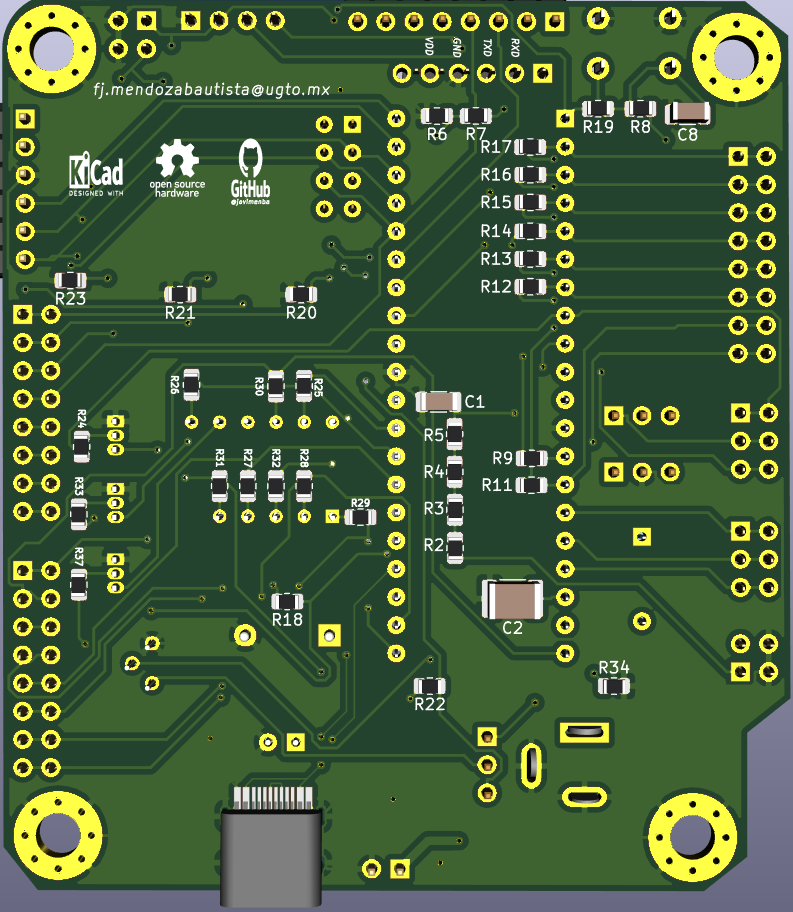
\includegraphics[width=4.3cm, height=4.3cm]{Img/tercera_version_pcb_b.png}
   % \caption{Segunda imagen.}
    %\label{fig:f23}
  \end{subfigure}
    \hspace{0.7cm}
  \begin{subfigure}[b]{0.4\columnwidth}
     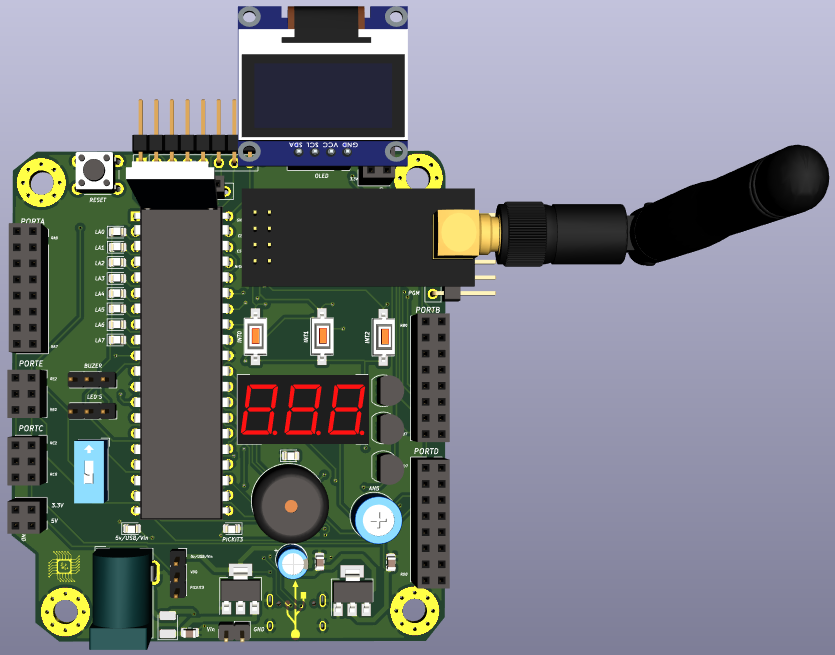
\includegraphics[width=4.3cm, height=4.3cm]{Img/tercera_version_3d.png}
    % \caption{Primera imagen.}
    %\label{fig:f13}
  \end{subfigure}
   \caption{\centering \textbf{Diseño y modelo 3D de circuito impreso Versión 3.0}} 
   \label{fig:11}
 \end{figure}



%\Img{7.9cm}{7.0cm}{tercera_version_3d}{Modelo 3D de circuito impreso Versión 3.0 capa superior}{fig:11}
%\Img{6.9cm}{6.0cm}{tercera_version_pcb_b}{Modelo 3D de circuito impreso Versión 3.0 capa inferior}{fig:11}
%-------------------------------------------------------------------------
%Resultados y discusión
\Section{Resultados y discusión}
La Versión 1.0 fue pensada para cumplir una única función adaptada a un sistema de alarma, la cual cumple satisfactoriamente. En cuanto a posibles fallas se encontró un sobrecalentamiento en un elemento del módulo de alimentación; se solucionó realizando una prueba de corto circuito para encontrar el origen de la falla en el elemento regulador LM7805. Es posible que esta pieza presentara un defecto de fabricación, por lo que se retiró dicho componente y se sustituyó por uno nuevo. En la Fig.~\ref{fig:12} se presenta un DEMO.
\Img{8.5cm}{7.0cm}{primera_version_demo}{Programa DEMO para Versión 1.0}{fig:12}
En la Versión 2.0 es importante resaltar que se consiguió agregar más elementos a la vez que se redujo el tamaño de la placa, resultado de utilizar SMD, es decir, incorporar elementos más pequeños nos permitió optimizar mejor el espacio de trabajo. El tamaño de los encapsulados rectangulares SMD que se utilizó en esta versión fue de 1206 (3.2 x 1.6
mm); se optó por estos por su fácil manipulación en el momento de ensamblaje. En la Fig.~\ref{fig:13} y Fig.~\ref{fig:14} se presenta un DEMO.
\Img{8.5cm}{7.0cm}{segunda_version_demoa}{Programa DEMO para Versión 2.0}{fig:13}
\Img{8.5cm}{7.0cm}{segunda_version_demob}{Programa DEMO para Versión 2.0}{fig:14}

En la Versión 3.0, y más reciente, se logró reducir el tamaño de los encapsulados rectangulares SMD a 0805 (2.0 x 1.25 mm); en consecuencia, la proporción del tamaño de la placa también se redujo. También se implementó un nuevo sistema de alimentación donde los elementos through hole(THT) que lo conformaban fueron sustituidos por componentes SMD y se cambió el grosor de las pistas en esta sección de la placa para aumentar su vida útil.

A partir de la Versión 1.0 se ha conseguido reducir el tamaño del circuito impreso gracias a la tecnología de fabricación de circuitos de doble cara, permitiendo optimizar el recurso; de la Versión 1.0 a 2.0 se redujo un 10.68\%, de la Versión 2.0 a 3.0 hasta un 37\%, y de la primera respecto a la última el resultado fue de 49.5\%. En otras palabras, esta placa consigue ser atractiva por su multifuncionalidad en diferentes campos de trabajo debido a que su tamaño le permite ser accesible y flexible.
%-------------------------------------------------------------------------
%Conclusiones
\Section{Conclusiones}
 El proyecto de las placas cumplió satisfactoriamente cada unos de los objetivos planteados a lo largo de este documento, las problematicas que surgieron en el diseño o durante la construcción se dieron solución sin comprometer la integridad de las placas de desarrollo.

El diseño de la versión 3, está pensado para que su vida útil sea el doble de las placas de desarrollo que se encuentran actualmente en el mercado y además su precio sea mucho menor.

Finalmente, considero que se debe motivar a las nuevas generaciones de estudiantes de Ingeniería Electrónica a profundizar en el diseño de circuitos
electrónicos y brindarles las herramientas necesarias para que sean capaces de realizar prácticas a nivel del ejercicio profesional y así generar un incremento en la producción de la zona y el país e ir al corriente con las tecnologías globales.

%
%-------------------------------------------------------------------------|
\begin{comment}
\Section{Instructions}

Please read the following carefully.

%------------------------------------------------------------------------- 
\SubSection{Language}

All manuscripts must be in English. Why?

%------------------------------------------------------------------------- 
\SubSection{Printing your paper}

Print your properly formatted text on high-quality, $8.5 \times 11$-inch 
white printer paper. A4 paper is also acceptable, but please leave the 
extra 0.5 inch (1.27 cm) at the BOTTOM of the page.

%------------------------------------------------------------------------- 
\SubSection{Margins and page numbering}

All printed material, including text, illustrations, and charts, must be 
kept within a print area 6-7/8 inches (17.5 cm) wide by 8-7/8 inches 
(22.54 cm) high. Do not write or print anything outside the print area. 
Number your pages lightly, in pencil, on the upper right-hand corners of 
the BACKS of the pages (for example, 1/10, 2/10, or 1 of 10, 2 of 10, and 
so forth). Please do not write on the fronts of the pages, nor on the 
lower halves of the backs of the pages.


%------------------------------------------------------------------------ 
\SubSection{Formatting your paper}

All text must be in a two-column format. The total allowable width of 
the text area is 6-7/8 inches (17.5 cm) wide by 8-7/8 inches (22.54 cm) 
high. Columns are to be 3-1/4 inches (8.25 cm) wide, with a 5/16 inch 
(0.8 cm) space between them. The main title (on the first page) should 
begin 1.0 inch (2.54 cm) from the top edge of the page. The second and 
following pages should begin 1.0 inch (2.54 cm) from the top edge. On 
all pages, the bottom margin should be 1-1/8 inches (2.86 cm) from the 
bottom edge of the page for $8.5 \times 11$-inch paper; for A4 paper, 
approximately 1-5/8 inches (4.13 cm) from the bottom edge of the page.

%------------------------------------------------------------------------- 
\SubSection{Type-style and fonts}

Wherever Times is specified, Times Roman may also be used. If neither is 
available on your word processor, please use the font closest in 
appearance to Times that you have access to.

MAIN TITLE. Center the title 1-3/8 inches (3.49 cm) from the top edge of 
the first page. The title should be in Times 14-point, boldface type. 
Capitalize the first letter of nouns, pronouns, verbs, adjectives, and 
adverbs; do not capitalize articles, coordinate conjunctions, or 
prepositions (unless the title begins with such a word). Leave two blank 
lines after the title.

AUTHOR NAME(s) and AFFILIATION(s) are to be centered beneath the title 
and printed in Times 12-point, non-boldface type. This information is to 
be followed by two blank lines.

The ABSTRACT and MAIN TEXT are to be in a two-column format. 

MAIN TEXT. Type main text in 10-point Times, single-spaced. Do NOT use 
double-spacing. All paragraphs should be indented 1 pica (approx. 1/6 
inch or 0.422 cm). Make sure your text is fully justified---that is, 
flush left and flush right. Please do not place any additional blank 
lines between paragraphs. Figure and table captions should be 10-point 
Helvetica boldface type as in
\begin{figure}[h]
   \caption{Example of caption.}
\end{figure}

\noindent Long captions should be set as in 
\begin{figure}[h] 
   \caption{Example of long caption requiring more than one line. It is 
     not typed centered but aligned on both sides and indented with an 
     additional margin on both sides of 1~pica.}
\end{figure}

\noindent Callouts should be 9-point Helvetica, non-boldface type. 
Initially capitalize only the first word of section titles and first-, 
second-, and third-order headings.

FIRST-ORDER HEADINGS. (For example, {\large \bf 1. Introduction}) 
should be Times 12-point boldface, initially capitalized, flush left, 
with one blank line before, and one blank line after.

SECOND-ORDER HEADINGS. (For example, {\elvbf 1.1. Database elements}) 
should be Times 11-point boldface, initially capitalized, flush left, 
with one blank line before, and one after. If you require a third-order 
heading (we discourage it), use 10-point Times, boldface, initially 
capitalized, flush left, preceded by one blank line, followed by a period 
and your text on the same line.

%------------------------------------------------------------------------- 
\SubSection{Footnotes}

Please use footnotes sparingly%
\footnote
   {%
     Or, better still, try to avoid footnotes altogether.  To help your 
     readers, avoid using footnotes altogether and include necessary 
     peripheral observations in the text (within parentheses, if you 
     prefer, as in this sentence).
   }
and place them at the bottom of the column on the page on which they are 
referenced. Use Times 8-point type, single-spaced.


%------------------------------------------------------------------------- 
\SubSection{References}

List and number all bibliographical references in 9-point Times, 
single-spaced, at the end of your paper. When referenced in the text, 
enclose the citation number in square brackets, for example~\cite{ex1}. 
Where appropriate, include the name(s) of editors of referenced books.

%------------------------------------------------------------------------- 
\SubSection{Illustrations, graphs, and photographs}

All graphics should be centered. Your artwork must be in place in the 
article (preferably printed as part of the text rather than pasted up). 
If you are using photographs and are able to have halftones made at a 
print shop, use a 100- or 110-line screen. If you must use plain photos, 
they must be pasted onto your manuscript. Use rubber cement to affix the 
images in place. Black and white, clear, glossy-finish photos are 
preferable to color. Supply the best quality photographs and 
illustrations possible. Penciled lines and very fine lines do not 
reproduce well. Remember, the quality of the book cannot be better than 
the originals provided. Do NOT use tape on your pages!

%------------------------------------------------------------------------- 
\SubSection{Color}

The use of color on interior pages (that is, pages other
than the cover) is prohibitively expensive. We publish interior pages in 
color only when it is specifically requested and budgeted for by the 
conference organizers. DO NOT SUBMIT COLOR IMAGES IN YOUR 
PAPERS UNLESS SPECIFICALLY INSTRUCTED TO DO SO.

%------------------------------------------------------------------------- 
\SubSection{Symbols}

If your word processor or typewriter cannot produce Greek letters, 
mathematical symbols, or other graphical elements, please use 
pressure-sensitive (self-adhesive) rub-on symbols or letters (available 
in most stationery stores, art stores, or graphics shops).

%------------------------------------------------------------------------ 
\SubSection{Copyright forms}

You must include your signed IEEE copyright release form when you submit 
your finished paper. We MUST have this form before your paper can be 
published in the proceedings.

%------------------------------------------------------------------------- 
\SubSection{Conclusions}

Please direct any questions to the production editor in charge of these 
proceedings at the IEEE Computer Society Press: Phone (714) 821-8380, or 
Fax (714) 761-1784.
\end{comment}
%------------------------------------------------------------------------- 
\nocite{ex1,ex2,ex3,ex4}
\bibliographystyle{latex8}
\bibliography{latex8}

\end{document}
